Nástrojů jak dnes psát dokumenty máme celou řadu, některé jsou volně dostupné a jiné jsou zpoplatněny. Některé nástroje jsme si již představili (Word, LibreOffice), ale
nyní se zaměříme na takzvané značkovací jazyky. Značkovací jazyky nám umožnují psát text, který je poté možné zpracovat počítačem, který změní jeho formátování. Většina
značkovacích jazyků má jasně rozlišitelné značky, nebo jinak také tagy, které upravují formátování při jejich strojovém překladu, díky tomu je původní text stále dobře čitelný.
\cite{markup}

Mezi značkovací jazyky například patří i jazyky používané při psaní webových stránek, jako je \gls{html} či \gls{xml}, ovšem tyto jazyky budeme spíše využívat pro zobrazování výstupu
jednodušších značkovacích jazyků jako je například Markdown.

\section{Markdown}

Markdown je značkovací jazyk, který převádí text do \gls{html}. Jedná se o jednoduše čitelný a zároveň jednoduchý jazyk na psaní strukturovaného textu. Hlavní myšlenkou Markdown je, že
text v něm psaný by měl být publikovatelný i bez jeho zpracování, inspirací tomuto přístupu jsou čistě textové emaily (emaily se dnes ve většině případů píšou v \gls{html}
z důvodu grafického obsahu). \cite{markdown}

Markdown se používá v na některých verzovacích službách jako je například Github, ovšem v tomto případě se jedná o upravenou implementaci Markdown, která je rozšířena o další
tagy/značky. Podobnou úpravu Markdown má i konkurenční služba GitLab.

Takto vypadá menší ukázka Markdown syntaxe a také výsledek, který je poté generován \ref{fig:markdown}.

\clearpage

\begin{minted}{md}
    # Ukázkový příklad Markdown syntaxe

    Takto vypadá dokument psaný v Markdown,
    jak je vidět, od čistého textu se moc neliší.

    ## Víceúrovňové nadpisy

    *kurzíva*, **tučné**, ~~přeskrtnuní~~

    - příklad
    - jednoduchého
    - seznamu

    - [ ] Checkbox
\end{minted}

\begin{figure}[h]
    \centering
    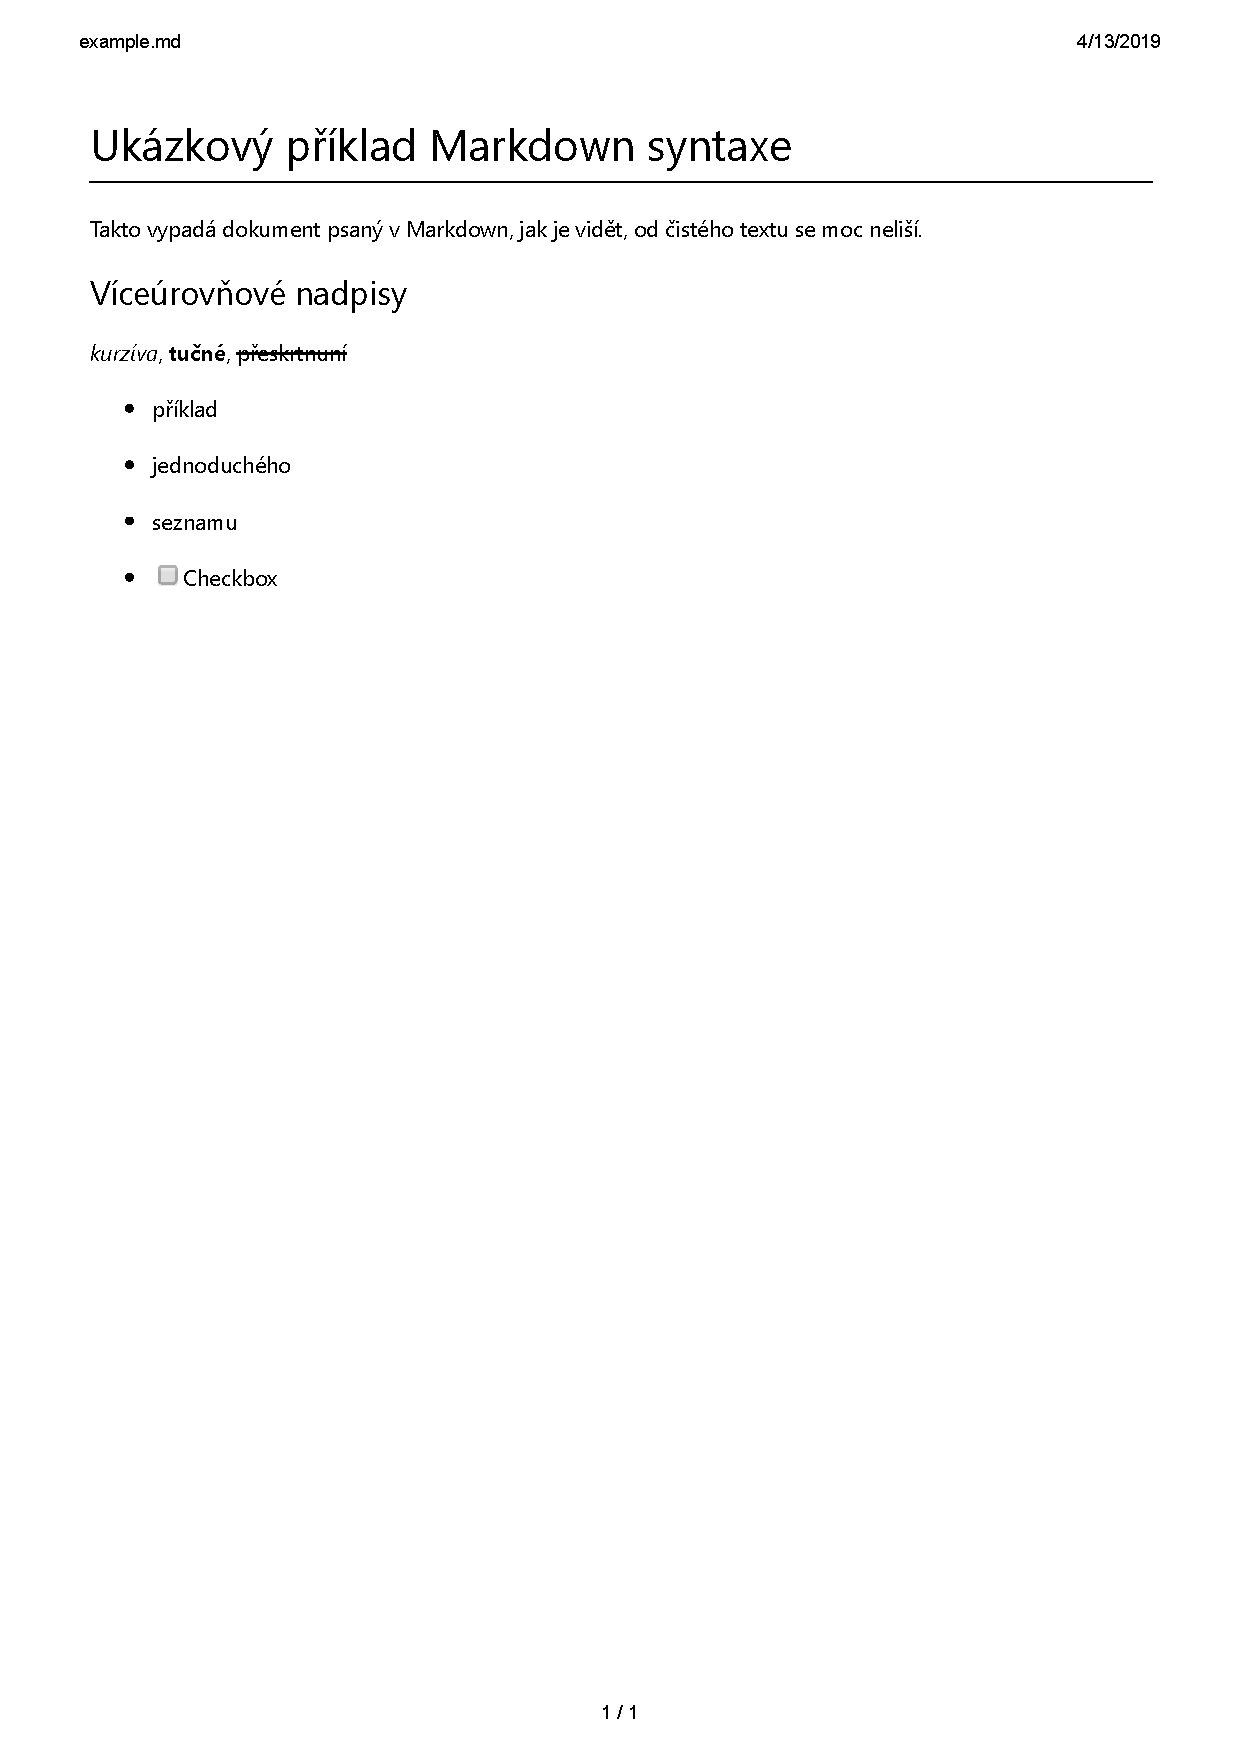
\includegraphics[width=\textwidth]{example.pdf}
    \caption{Výstup Markdown}
    \label{fig:markdown}
\end{figure}

\section{reStructuredText}

Formát reStructuredText pro psaní dokumentů v prostém textu, který je jednoduchý na čtení, kde je hned zřejmé jak bude vygenerovaný text vypadat.
Tento formát je jednoduchý na použití hlavně pro psaní programátorské dokumentace, jednoduchých webů a samostatných dokumentů.
Hlavním cílem reStructuredText je definovat a uplatnit jednoduchý značkovací jazyk pro použítí v Python, kde se používá k dokumentaci jednotlivých částí programu,
a dalších dokumentačních nástrojích, který je jednoduše čitelný a jednoduše použitelný. \cite{reStruDoc}

Docutil podporuje formát reStructuredText, proto jej v rámci teto sekci lehce představme.
\uv{Docutil je open-source program pro zpracovaní dokumentace v textové podobě do, pro uživatele, přívětivého formátu, jako je například \gls{html}, \LaTeX~či \gls{xml}.} \cite{docutil}
Díky využití reStructuredText se tedy jedná o nástroj na tvorbu modulárních dokumentů, ovšem tento nástroj je určen spíše pro programátory na vytváření dokumentace a nehodí se
pro běžného uživatele.

\inputminted{rst}{example-rst.rst}

\begin{figure}[h]
    \centering
    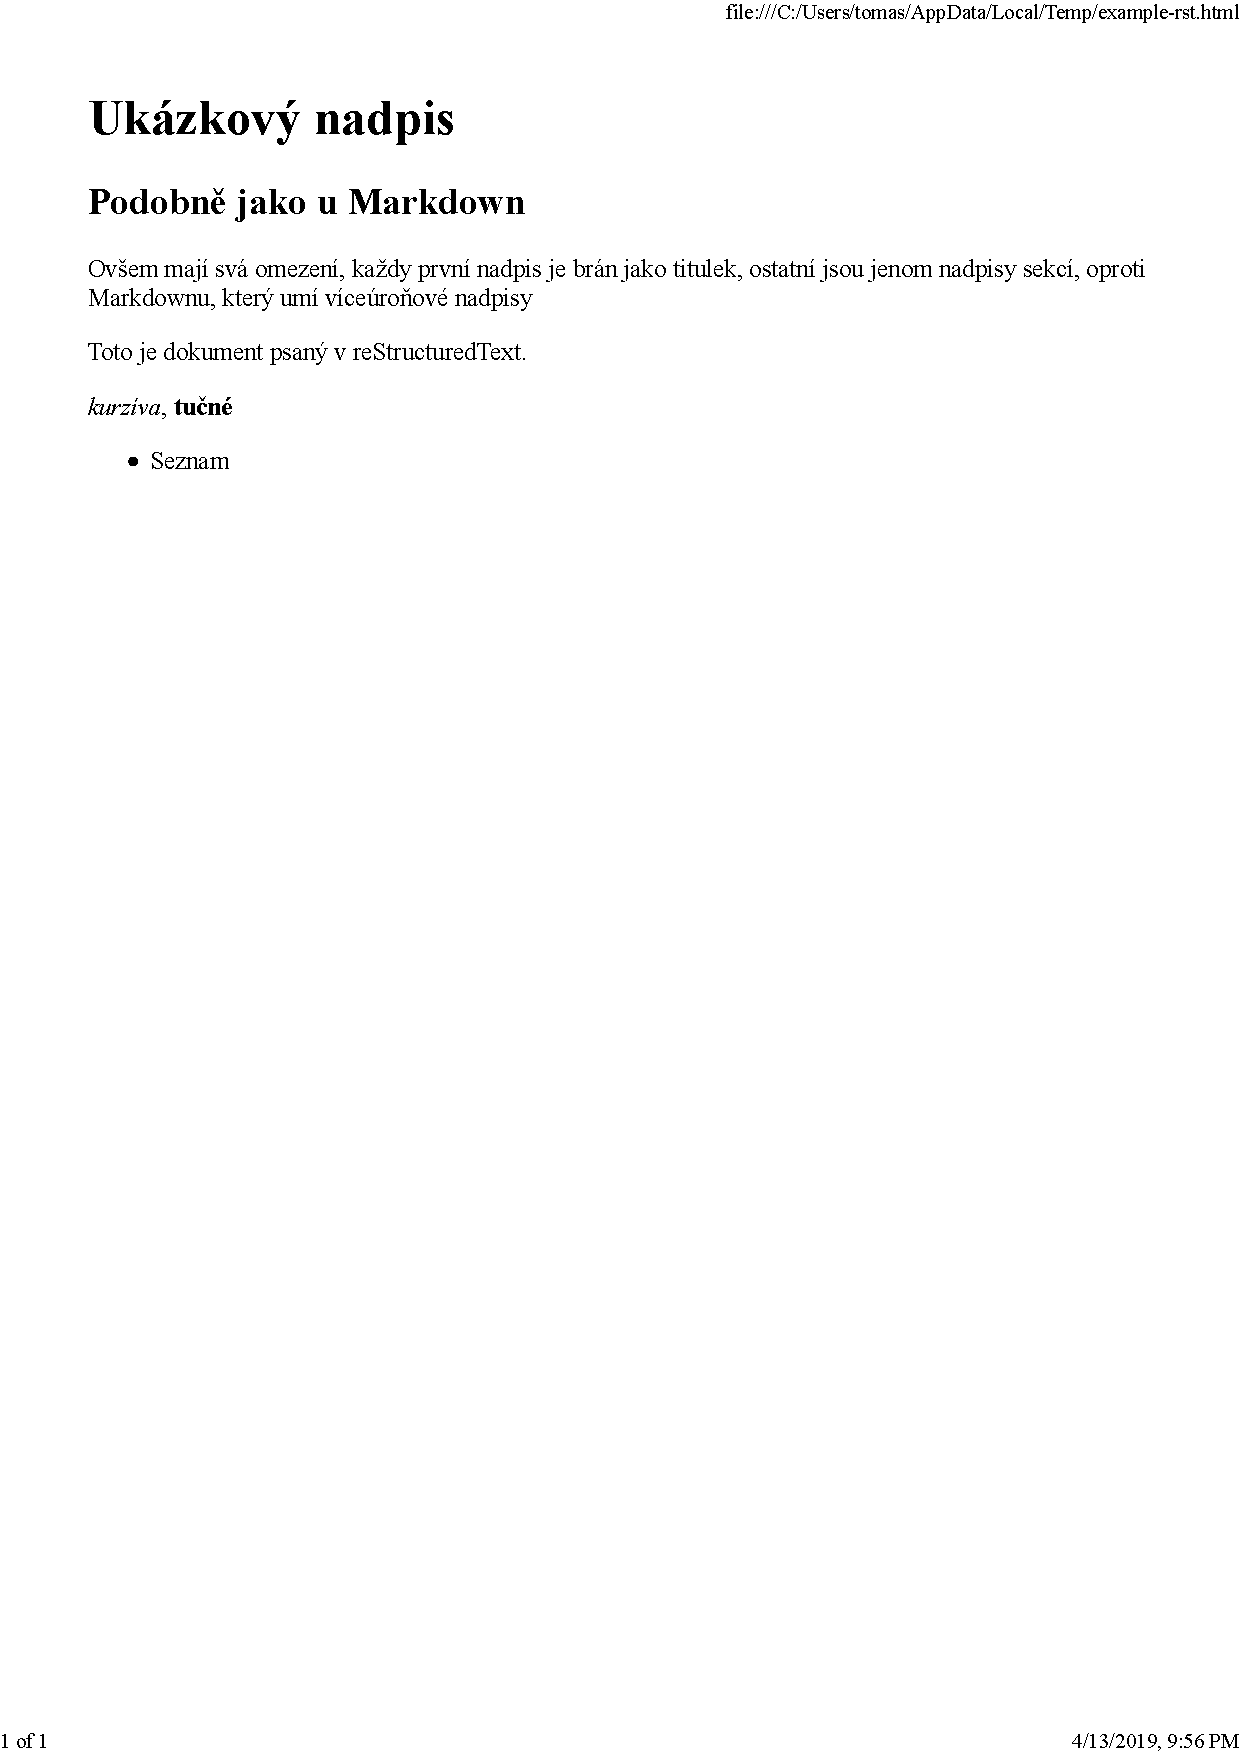
\includegraphics[width=\textwidth]{example-rst.pdf}
    \caption{Výstup reStructuredText}
    \label{fig:rstOutput}
\end{figure}

\section{AsciiDoc}

AsciiDoc je další formát pro psaní dokumentu, jedná se stejně jako reStructuredText, o modul pro jazyk Python. Tento modul je možné použít pro psaní nejenom poznámek,
ale je možné jej exportovat i do formátů jako jsou .epub (formát pro elektronické čtečky knih), či PDF. \cite{asciiDoc} Syntaxe jazyku je podobná reStructuredText.

Projekt byl původně psán pro jazyk python, ovšem posléze byla syntaxe adoptována jako balíček pro jazyk ruby a také přejmenován na AsciiDoctor.

\inputminted{text}{example-ascii.adoc}
\todo{better sample text}

\section{Porovnání}

Po představení těchto 3 značkovacích jazyků je na čase si je zhodnotit vzhledem k této práci a vybrat z nich ten, který poté použijeme v rámci implementace.

\begin{figure}[h]
    \centering
    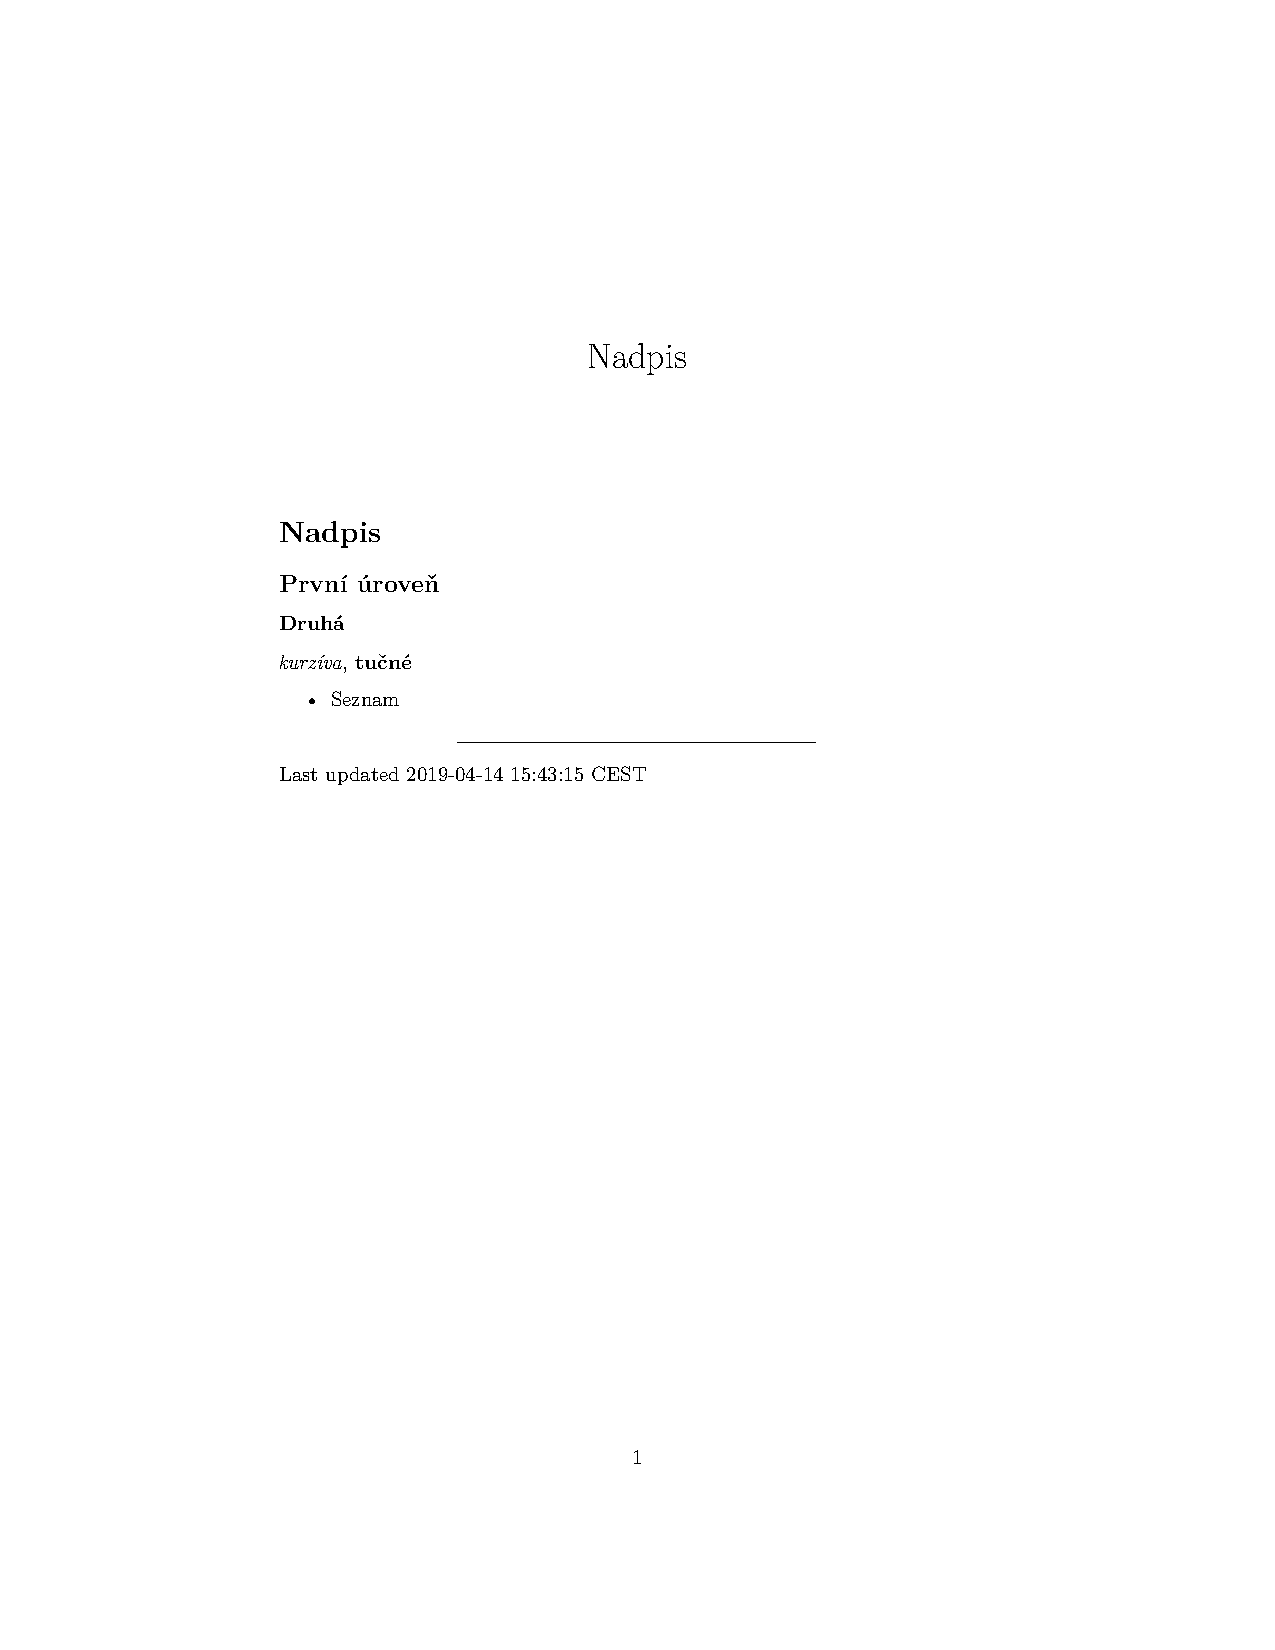
\includegraphics[width=\textwidth]{example-ascii.pdf}
    \caption{Výstup AsciiDoc}
    \label{fig:asciiOutput}
\end{figure}
